\documentclass[12pt]{article}

\usepackage[utf8]{inputenc}
\usepackage{geometry}
\geometry{a4paper,scale=0.75}
\linespread{1.5}
\usepackage{graphicx} 
\usepackage{float} 
\usepackage{subfig} 
\usepackage{enumerate}
\usepackage{enumitem}
\usepackage{amsmath}
\usepackage{array}
\usepackage{booktabs}
\usepackage{multirow}
\usepackage{amsfonts}
\usepackage[english]{babel}
\usepackage{amsthm}
\usepackage{dcolumn}
\usepackage{multicol}
\usepackage{stfloats}
\usepackage{lscape}
\usepackage[figuresright]{rotating}
\RequirePackage{pdflscape}
\usepackage[toc,page]{appendix}
\usepackage{geometry}
\usepackage{longtable}
\usepackage{comment}
\usepackage{xcolor}

% -------- enumerated sub-labels (a), (b), … --
\usepackage{enumitem}
\setlist[enumerate,1]{label=(\alph*),ref=\alph*}
% ---------------------------------------------

\usepackage{hyperref}
\hypersetup{hidelinks,
	colorlinks=true,
	allcolors=black,
	pdfstartview=Fit,
	breaklinks=true}
\usepackage{csquotes}
\usepackage{natbib}
\bibliographystyle{apalike}
\newtheorem{definition}{Definition}
\newtheorem{theorem}{Theorem}
\newtheorem{proposition}[theorem]{Proposition}
\newtheorem{lemma}[theorem]{Lemma}
\newtheorem{corollary}[theorem]{Corollary}
\newtheorem*{remark}{Remark}
\newtheorem{example}{Example}
\newtheorem{exercise}{Exercise}
\newtheorem{assumption}{Assumption}[section] % number within sections


\begin{document}

\begin{center}
    ECON 3123: Macroeconomic Theory I\\
    {\large \textbf{Tutorial Note 4: IS-LM Framework}}\\
    Teaching Assistant: Harlly Zhou
\end{center}

\subsection*{Basic IS-LM Model}
\paragraph{Deriving the Model}
Recall that in the goods market, the deamnd for goods is
\[ Z = C + I + G. \]
Recall that consumption depends on disposable income $Y-T$. And in reality, investment depends on output and interest rate:
\[ I = I (Y,i),\]
where $I$ increases with $Y$ and decreases with $i$. (Think about the intuition.)

Then we rewrite the demand as
\[ Z = C(Y-T) + I(Y,i) + G.\]
At equilibrium, we have
\[ Y = Z.\]
This determines the equilibrium output $Y^*$. When the nominal interest rate increases, the investment will decrease, shifting the $ZZ$ curve downwards. We have the new equilibrium output $Y'$, shown as Figure \ref{fig:is_01}.

\begin{figure}[htp]
    \centering
    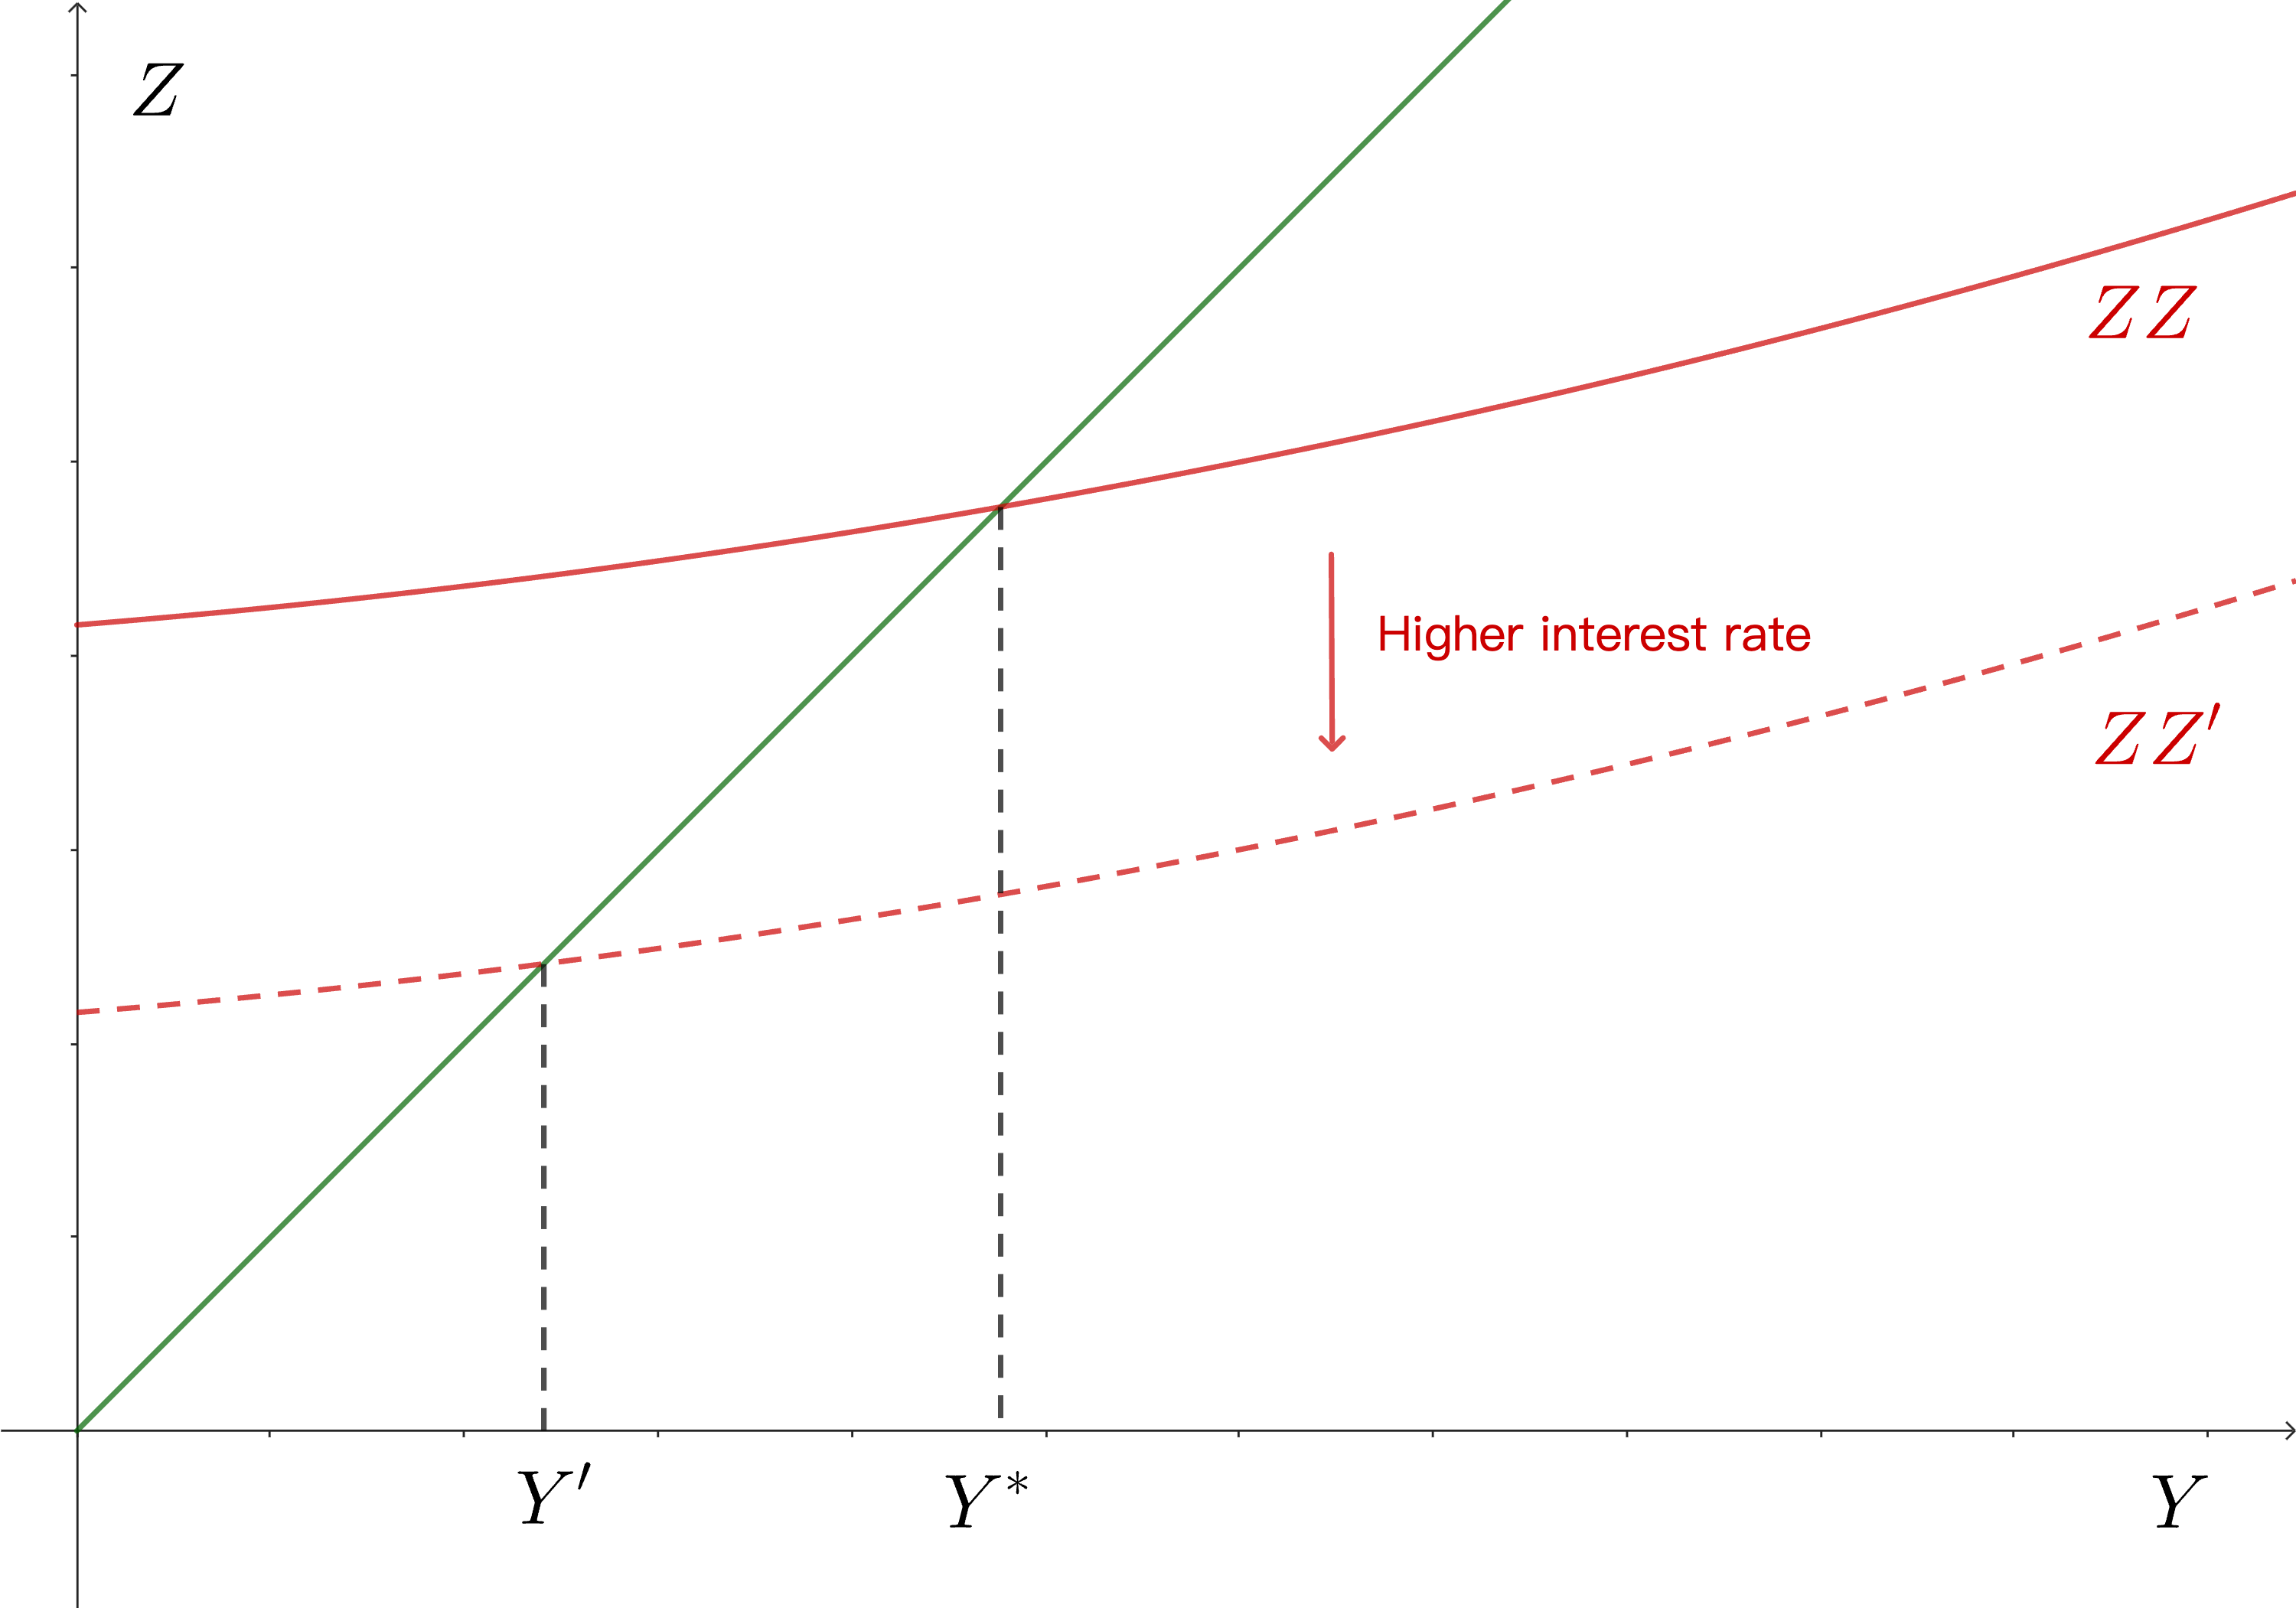
\includegraphics[width=0.6\textwidth]{is_01.png}
    \caption{Goods Market Equilibrium}
    \label{fig:is_01}
\end{figure}

If we put the interest rate and the output together, then we get the IS relation (Figrue \ref{fig:is_02}).\

\begin{figure}[htp]
    \centering
    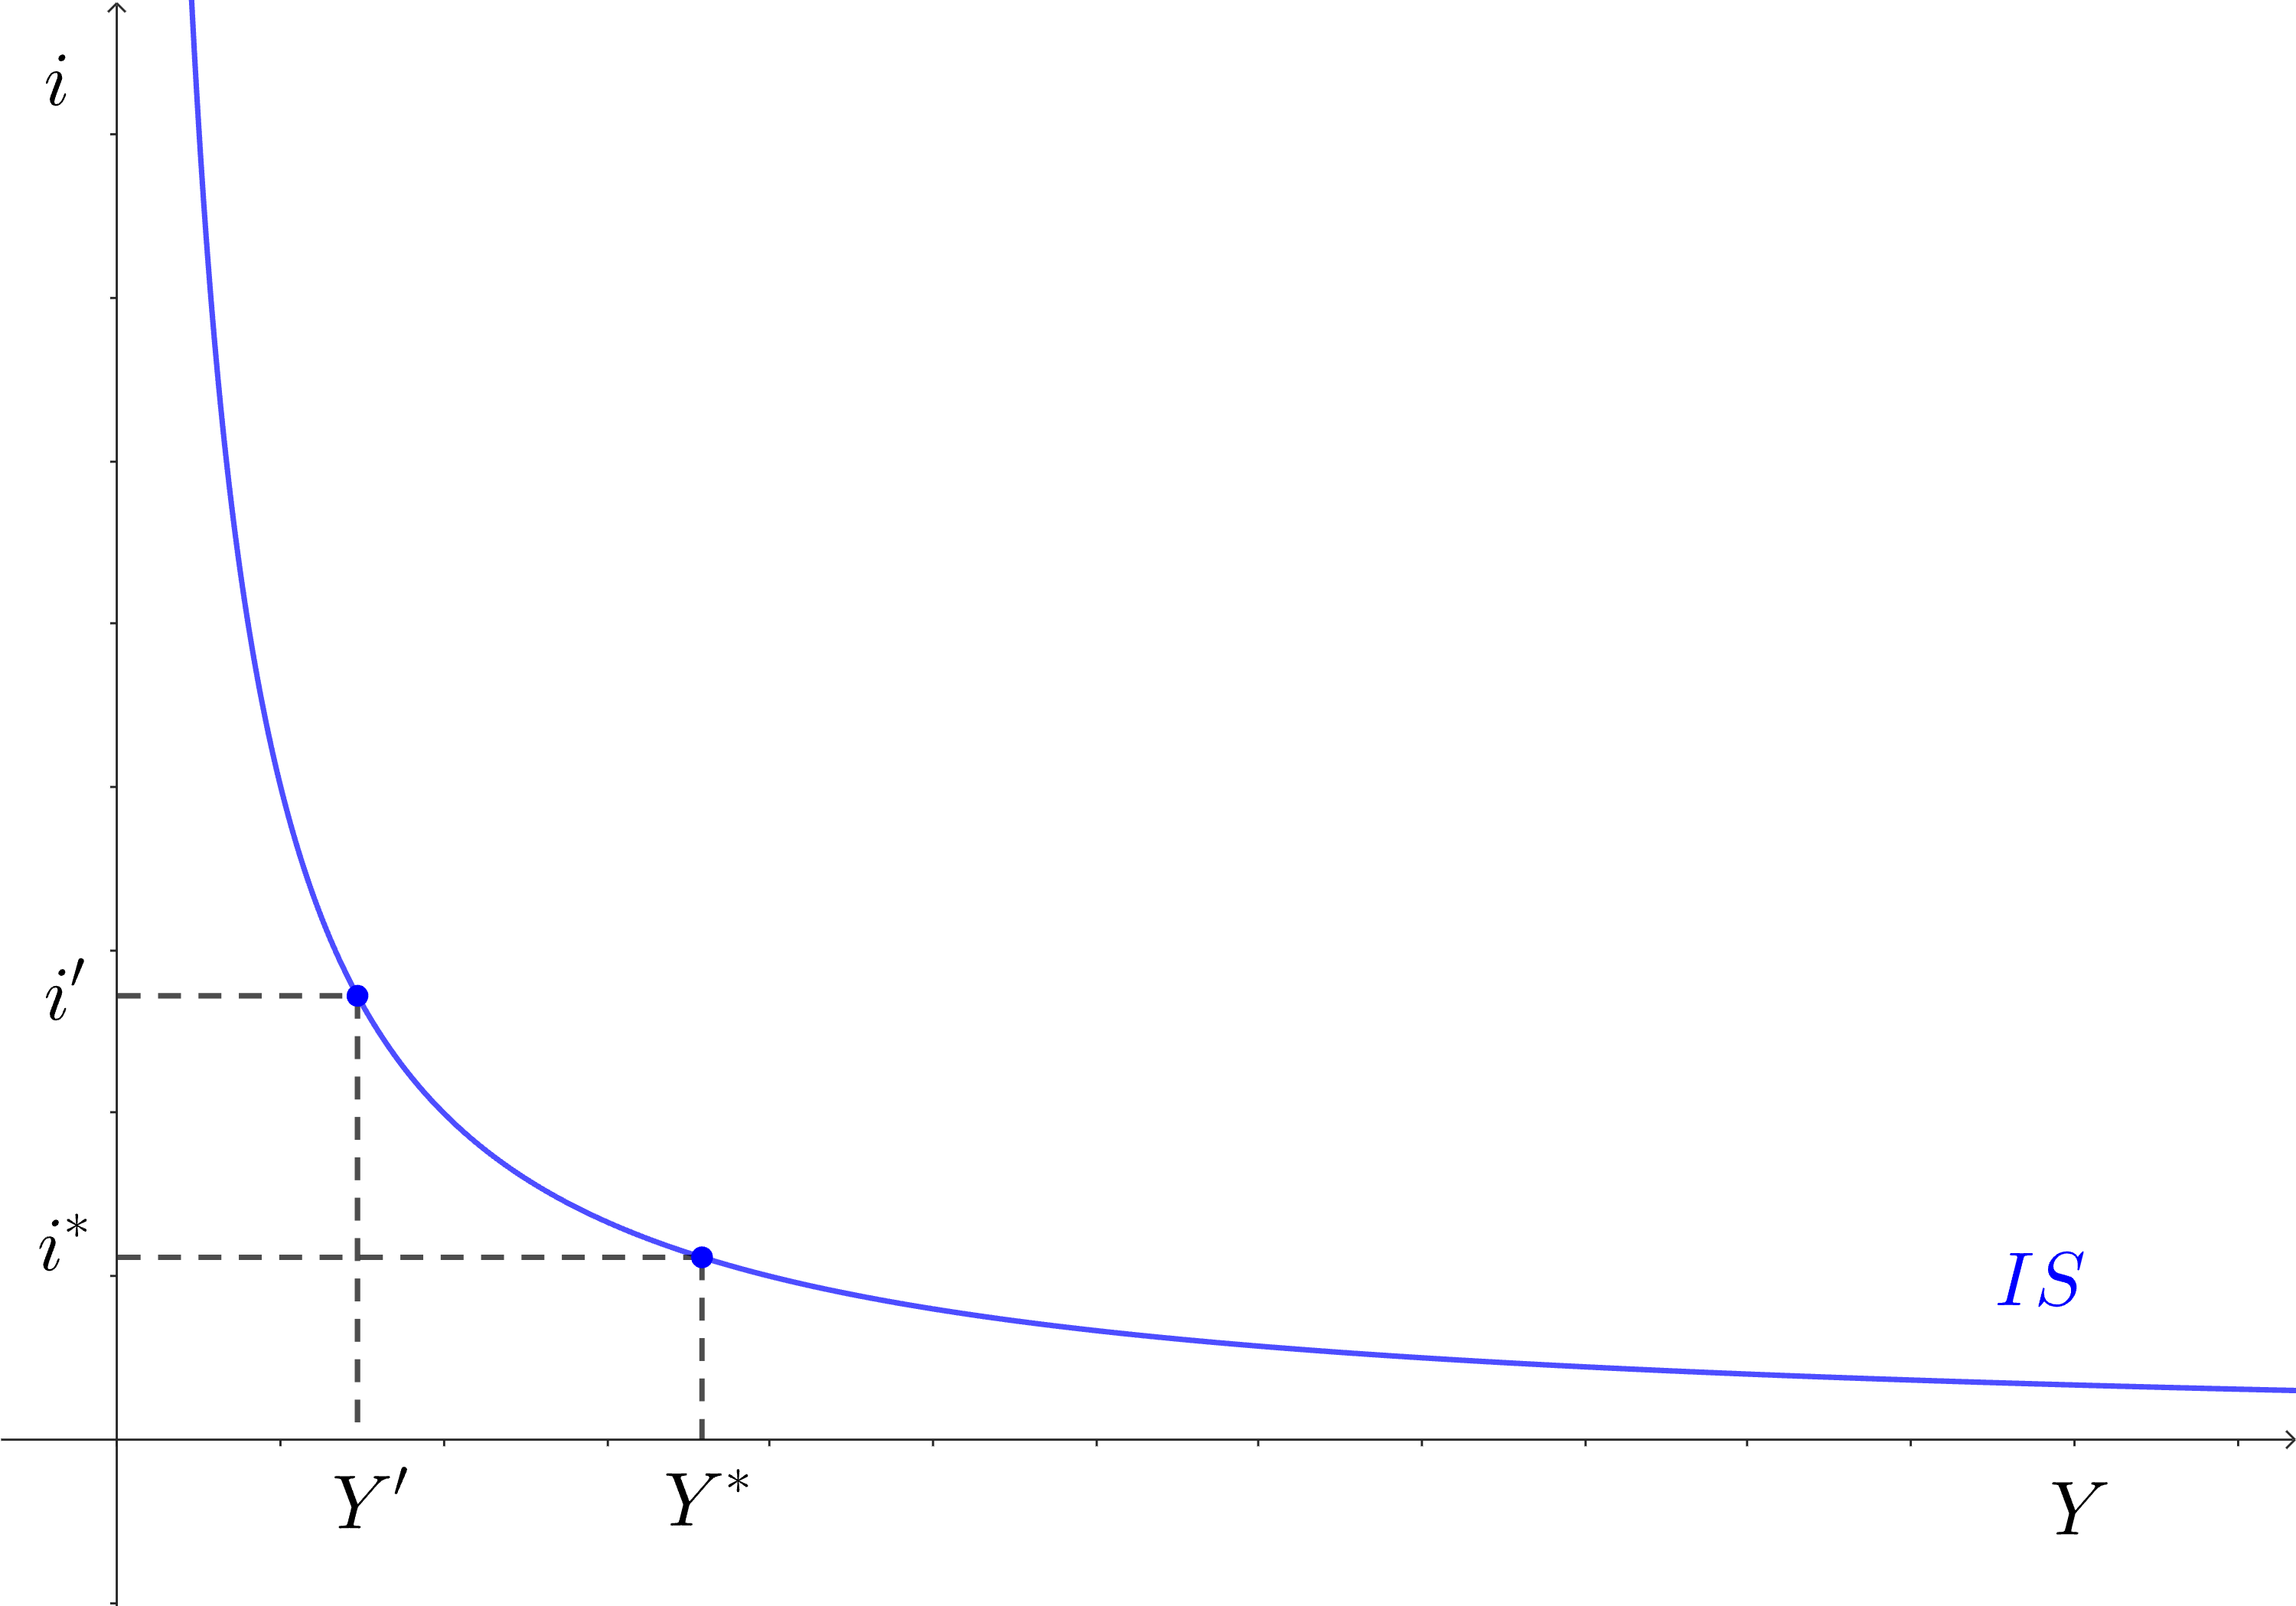
\includegraphics[width=0.6\textwidth]{is_02.png}
    \caption{Deriving IS curve from goods market equilibrium}
    \label{fig:is_02}
\end{figure}

Note that all the pairs $(i, Y)$ is a pair of \textbf{equilibrium} values of nominal interest and output.

In the derivation of the IS relation, note that the output is measured in \textit{real temr}. Therefore, we should also use real term in the money market equilibrium to derive the \textbf{LM relation}. Recall that the nominal money demand is
\[M^d = \$ Y L(i)\]
for some decreasing function $L(i)$. The real money demand is
\[\frac{M^d}{P} = Y L(i).\]
At equilibrium, $M^d = M^S = M$. In the short run, we assume that prices are sticky. Hence, we have
\[ \frac{M}{P} = Y L(i).\]
Central banks adjust money supply $M$ to target an interest rate $i = \bar{i}$. Hence, the LM curve is a horizontal line. Putting together with the IS curve, we get Figure \ref{fig:is-lm}.

\begin{figure}[htp]
    \centering
    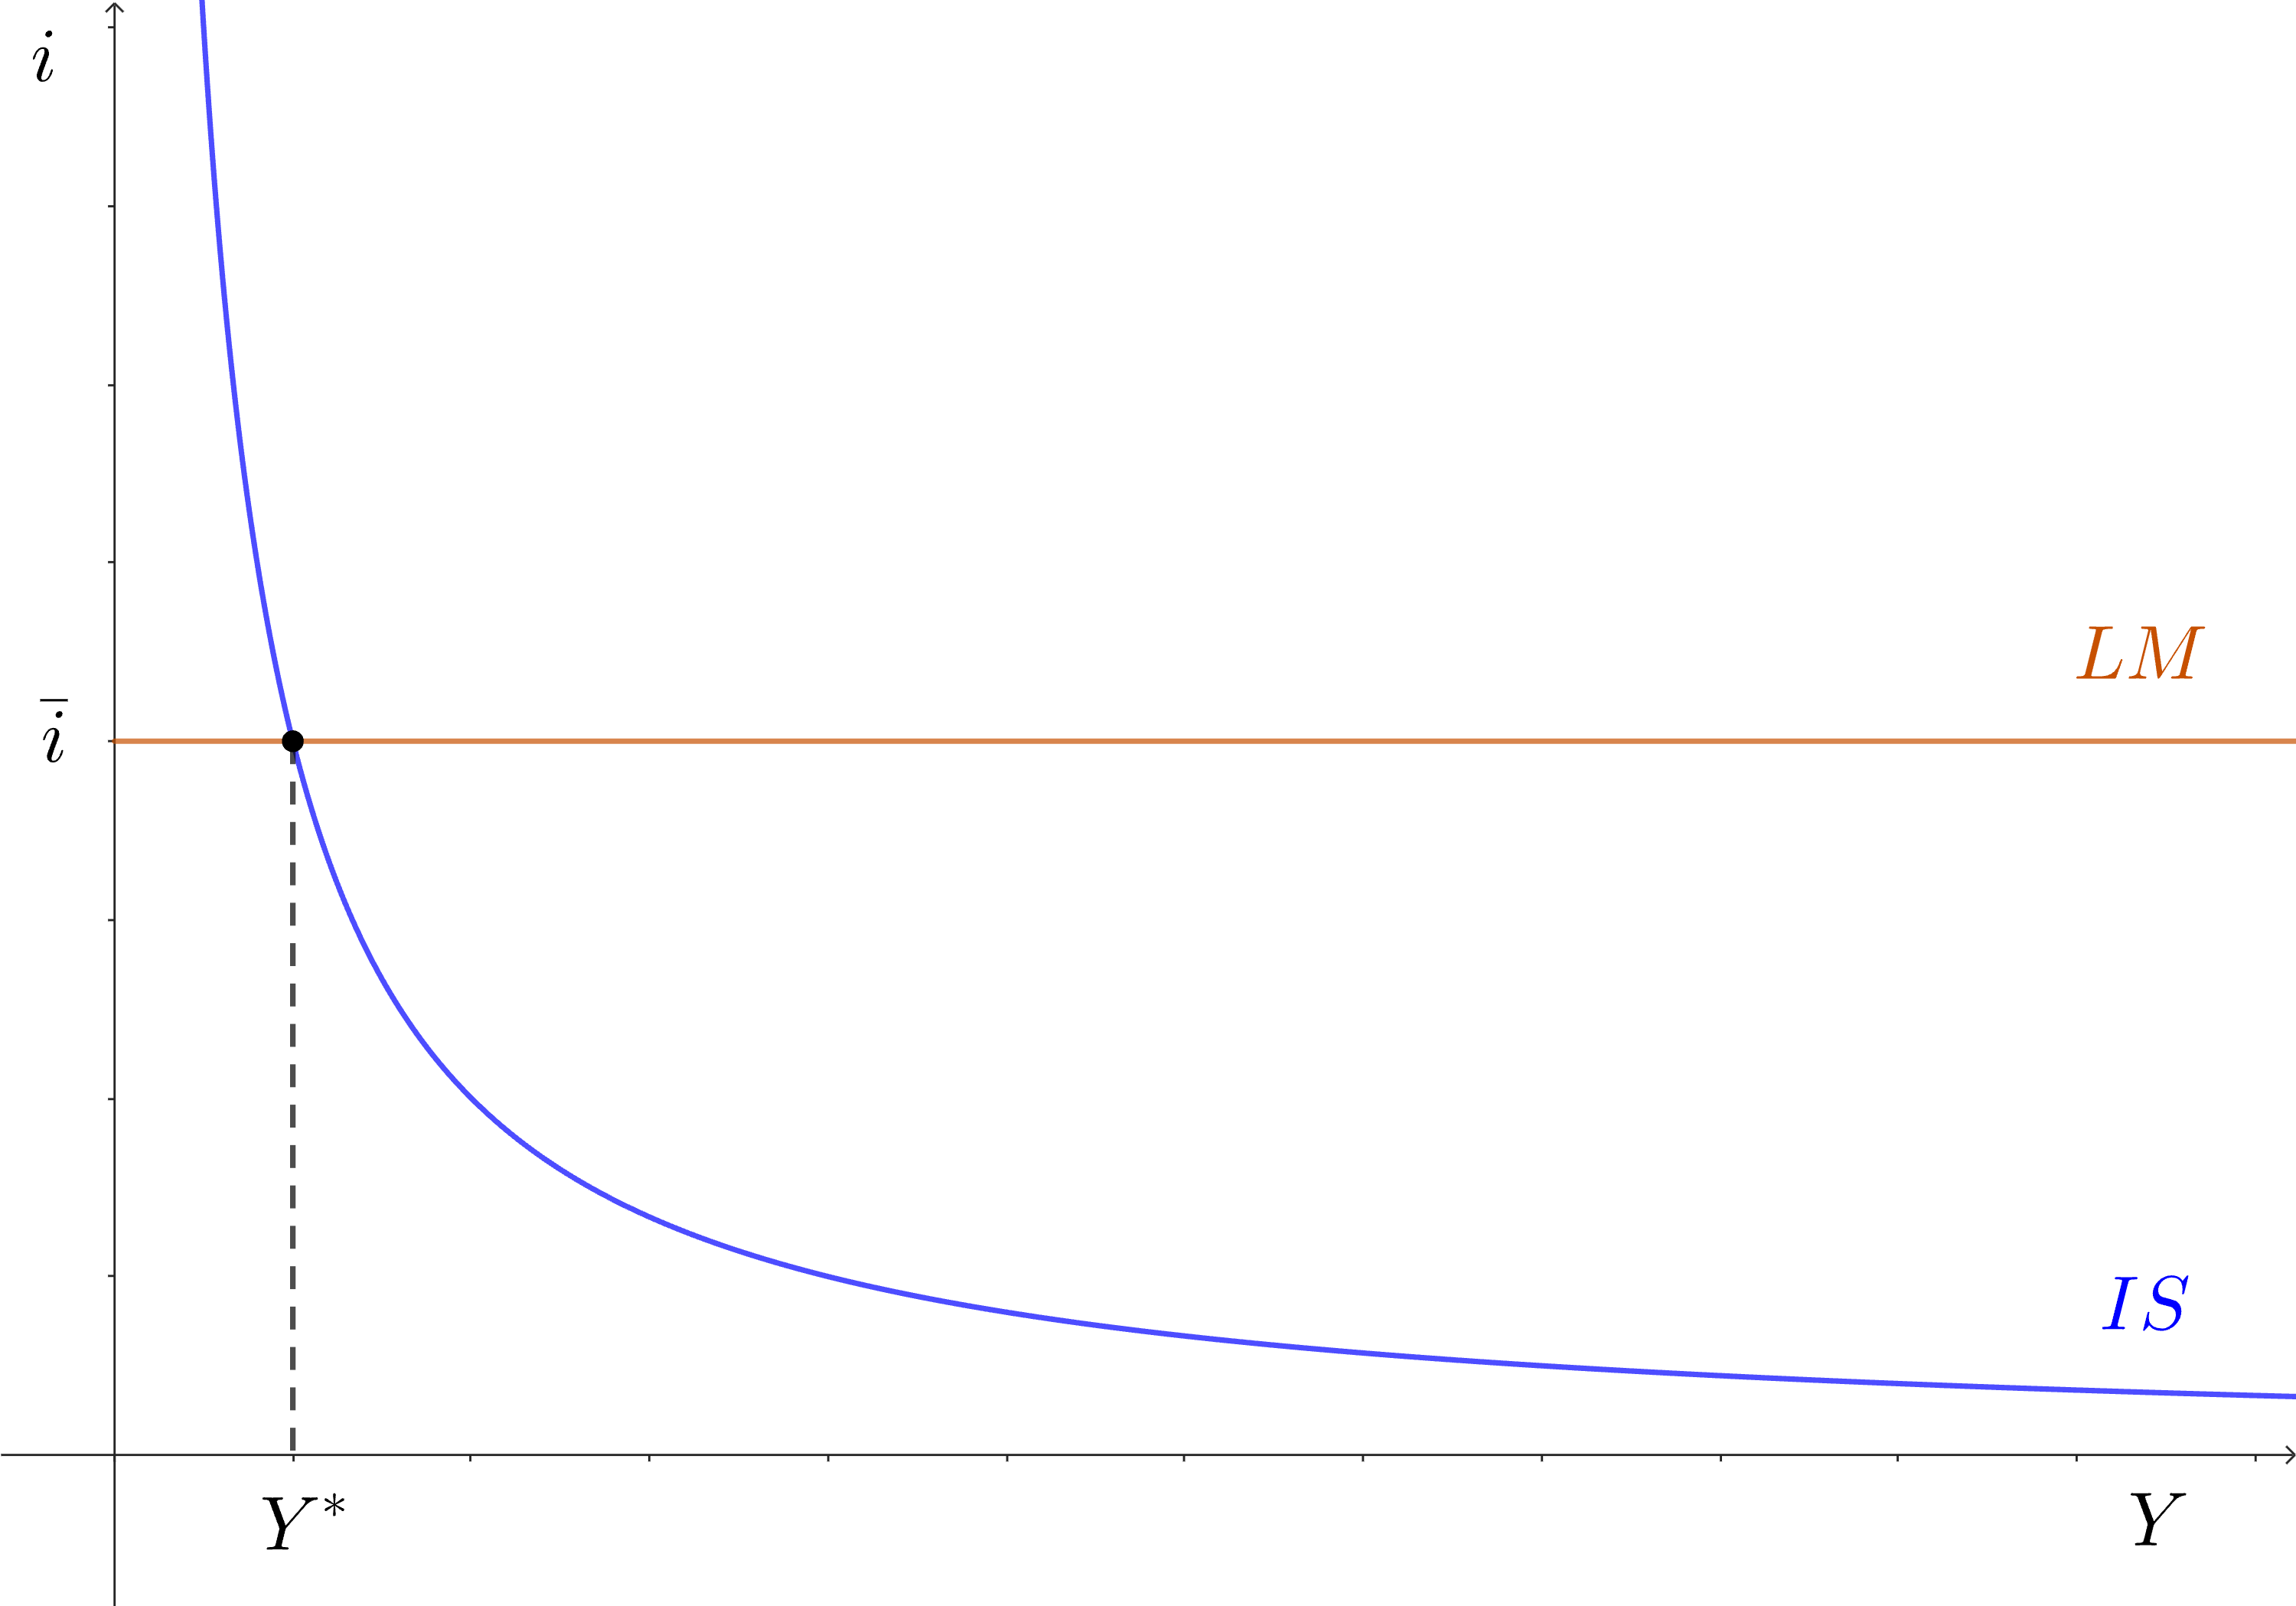
\includegraphics[width=0.6\textwidth]{is-lm.png}
    \caption{IS-LM Framework}
    \label{fig:is-lm}
\end{figure}

They together yield the \textbf{general equilibrium} interest rate and output, $(\bar{i}, Y^*)$.

\begin{exercise}
    Chapter 5, Question 5 in Blanchard, Olivier (2021), \textit{Macroeconomics}, 8th ed., Pearson.
\end{exercise}

\begin{exercise}
    \begin{enumerate}[label=(\arabic*)]
        \item At a given interest rate level, a temporary reduction in government purchases will
        \begin{enumerate}[label=\Alph*.]
            \item increase desired saving, causing the IS curve to shift down and to the left.
            \item increase desired saving, causing the IS curve to shift up and to the right.
            \item decrease desired saving, causing the IS curve to shift down and to the left.
            \item decrease desired saving, causing the IS curve to shift up and to the right.
        \end{enumerate}
        \item When all markets in the economy are simultaneously in equilibrium, we say
        \begin{enumerate}[label=\Alph*.]
            \item markets are complete.
            \item markets are perfect.
            \item there is disequilibrium.
            \item there is general equilibrium.
        \end{enumerate}
        \item If government spending and taxes increase by the same amount, the IS curve will
        \begin{enumerate}[label=\Alph*.]
            \item shift to the left.
            \item shift to the right.
            \item stay unchanged.
            \item have an ambiguous shift.
        \end{enumerate}
    \end{enumerate}
\end{exercise}

\begin{example}
    Suppose that the consumption behavior of people follows:
    \begin{align*}
        C = 0.8 (Y-300)
    \end{align*}
    and the investment follows:
    \begin{align*}
        I= aY + 510 - 200 i,
    \end{align*}
    where $a$ is a constant. Suppose that government spending is 300, total export is 200, total import is 400, and the price level is 10.

    Suppose that the nominal money demand is
    \begin{align*}
        M^d = \$ Y (0.25 - i),
    \end{align*}
    and the government is targeting a nominal interest rate of $5\%$.

    \begin{enumerate}[label=(\arabic*)]
        \item Let $a=0.1$. Derive the IS relation and the LM relation. Use the IS-LM framework to derive the equilibirum output.
        \item Keep $a=0.1$. Instead of targeting a nominal interest rate of $5\%$, the central bank starts to target $4\%$. How will the equilibrium consumption change?
        \item Can we have $a=0.2$? Explain. 
    \end{enumerate}
\end{example}

\paragraph{Policy Analyses Exercises}
\begin{example}
    Consider an economy like Argentina in 2001. Due to rampant corruption from the government, massive tax evasion, and money laundering activities, both consumers and investors become very pessimistic about the Argentine economy. Suppose initially, the economy is in an equilibrium. Use figures to answer the questions together with concise explanation.
    \begin{enumerate}[label=(\arabic*)]
        \item Explain what happens to the economy in the short run when people become pessimistic about the economy. What will happen to output and the real interest rate?
        \item If you are the government of Argentina, what would you do with government spending in order to offset the effects of the pessimism? What will happen to output, the real interest rate, price level, investment, and the consumption as the result of the government's action?
        \item If you are the central bank of Argentina, what kind of monetary policy that you can implement in order to offset the effects of the pessimism? What will happen to output, the real interest rate, price level, investment, and the consumption as the result of the central ban's action?
        \item Suppose the Argentine government has very limited fiscal space, and it is already running very high budget deficit so that the government is very likely to default on its debt, and simultaneously, the nominal interest rate in Argentina is very close to zero, or the zero lower bound (ZLB). 
        \begin{enumerate}[label=\alph*.]
            \item Is it still appropriate to use the policy suggested in part (2)? Why?
            \item Is it still appropriate to use the policy suggested in part (3)? Why?
            \item What kind of policies can be implemented in order to offset the effects of the pessimism? Please suggest at least 1 policy and explain why it works.
        \end{enumerate}
    \end{enumerate}
\end{example}

\subsection*{Introducing Financial Sector}
\paragraph{The Fisher Equation}
By no-arbitrage condition, we have
\[ 1 + r_t = \frac{(1 + i_t) P_t}{P^e_{t+1}}.\]
Since
\[\pi^e_{t+1} = \frac{P^e_{t+1}-P_t}{P_t},\]
we obtain
\[1 + r_t = \frac{1 + i_t}{1 + \pi^e_{t+1}}.\]
By an approximation, we obtain the \textbf{Fisher Equation}:
\[r_t \approx i_t = \pi^e_{t+1}.\]

\paragraph{Risk Premium}
To hedge the default risk, the bank always charge a risk premium $x$ other than the real rate for firm financing. Therefore, instead of having $I = I(Y,i)$, we have
\[ I = I (Y, r+x) = I(Y, i-\pi^e+x).\]

\begin{exercise}[No-arbitrage condition]
    David wants to borrow \$1,000 from Chris, and he says that the market rate is 5\%. Since David and Chris are friends, Chris would like to say yes to him. Victoria tells Chris to wait. She knows that David borrowed money from different people in the past for \$10,000 in total but only returned \$8,000 together with the interest. Chris are now hesitate on how much interest rate to charge him. What rate should Chris charge David to hedge for the default risk?
\end{exercise}
\end{document}